\section{Results}

 for several cases:
- not trusting/using  the EKF velocities
- trusting the EKF velocities
- using a single subsea position fix or multiple subsea range measurements to further constrain the output (I think only the nonlinear model can do this gracefully / easily?)
And then using ground truth from one of the mooring for comparison.

\begin{figure}%[!ht]
%  \centering
%  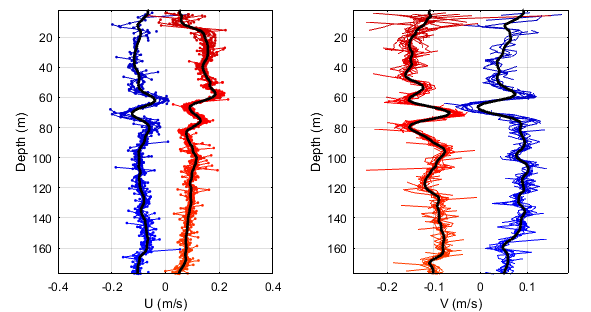
\includegraphics[width=\columnwidth]{./figs/current_profile_snip.png}
  \vspace{1.5in}
  \caption{The above plot shows a comparison of the results from the linear method with and without knowledge of the glider's through-the-water (TTW) velocity. On the left hand side is a snippet of the aligned individual traces and the resulting current estimate. On the right hand side is the resulting glider trajectory of a single candidate dive, in this case, dive \# XXX. The top plots show results produced without knowledge of the glider's TTW velocity (blue line), where the difference between overlapping traces is minimized while producing a current profile such that the glider ends up at the end-of-dive GPS. The lower plots show results produced when including knowledge of the glider's TTW velocity, in this case with a weighting of 0.8 (black line). This produces a more sensical glider trajectory in that...}
  \label{fig.linear}
\end{figure}


\begin{figure}%[!ht]
%  \centering
%  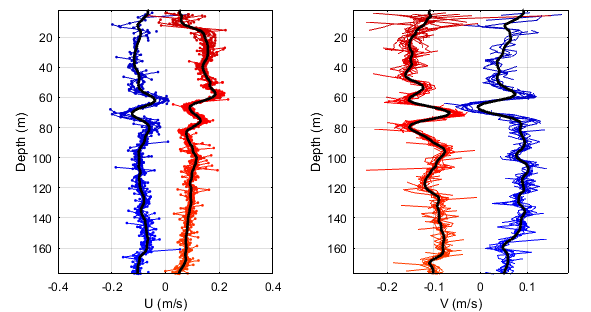
\includegraphics[width=\columnwidth]{./figs/current_profile_snip.png}
  \vspace{1.5in}
  \caption{The above plot shows a similar comparison as Figure \ref{fig.linear}, but for the nonlinear method...}
  \label{fig.nonlinear}
\end{figure}

\begin{figure}%[!ht]
%  \centering
%  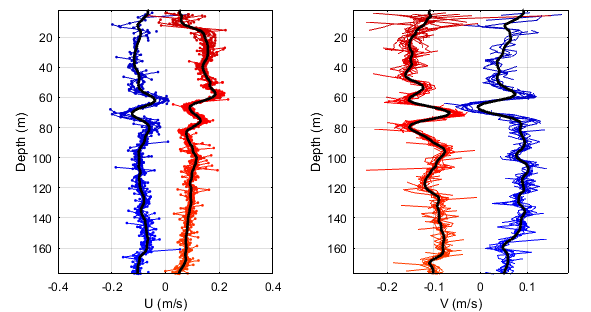
\includegraphics[width=\columnwidth]{./figs/current_profile_snip.png}
  \vspace{1.5in}
  \caption{The above plot shows a comparison between the the linear, nonlinear, and ground truth as obtained from a 300 kHz ADCP on the T4 mooring...}
  \label{fig.mooring}
\end{figure}


\begin{figure}%[!ht]
%  \centering
%  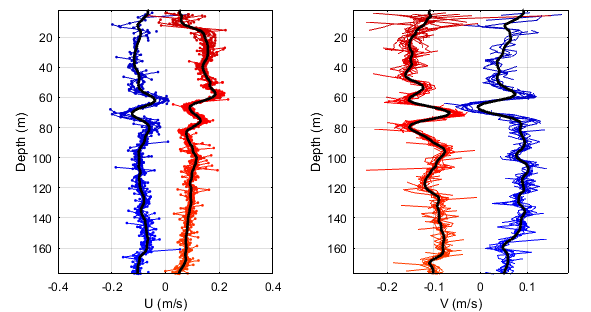
\includegraphics[width=\columnwidth]{./figs/current_profile_snip.png}
  \vspace{1.5in}
  \caption{The above plot shows the results from the nonlinear method, this time incorporating an additional subsea fix, arred at using 4 range measurements received over 37 minutes while the AUG was decending from 3042m and 581m. On the left is the current profile, compared to the ground truth from the mooring. On the right is the glider trajectory.}
  \label{fig.subseafix}
\end{figure}


% Figure \ref{fig.profile_snip} shows a short section of the dive with the individual ADCP profiles, offset by our initial estimate of the AUG's TTW velocity (i.e., the velocity from the hydrodynamic model, without accounting for current-induced motion). The thick black line is the estimated current profile. This is from a 750 m dive, so the sections of data shown were collected 3.5 hrs apart. The difference in the current profile during ascent and descent are clearly visible, motivating the need for different current profiles during ascent and descent.

% \begin{figure}[!ht]
%   \centering
%   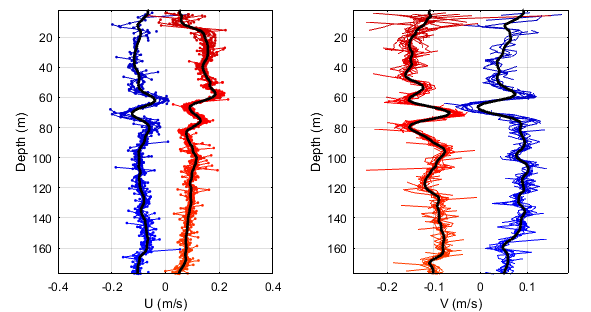
\includegraphics[width=\columnwidth]{./figs/current_profile_snip.png}
%   \vspace{-0.1in}
%   \caption{ Overlapped ADCP profiles during descent (blue) and ascent (red) for dive 116 of sg198. The fitted current profile is shown as the thick black line.}
%   \label{fig.profile_snip}
%   \vspace{-0.1in}
%   %\rule{\textwidth}{0.02in}
% %   \vspace{-0.2in}
% \end{figure}


\section{Conclusions and Future Work \textbf(SARAH)}


\section*{Acknowledgements \textbf(SARAH)}
We would like to acknowledge...
